%%%%%%%%%%%%%%%%%%%%% chapter.tex %%%%%%%%%%%%%%%%%%%%%%%%%%%%%%%%%
%
% sample chapter
%
% Use this file as a template for your own input.
%
%%%%%%%%%%%%%%%%%%%%%%%% Springer-Verlag %%%%%%%%%%%%%%%%%%%%%%%%%%
%\motto{Use the template \emph{chapter.tex} to style the various elements of your chapter content.}
\chapter{An Overview on IEEE 802.11/Wi-Fi Medium Access Control}
\label{overview-wifi}

%TODO: Abstract
\abstract{In order to understand and analyze the interactions between U-LTE and Wi-Fi in the $5$ GHz frequency band, knowledge on the architectures and Medium Access Control (MAC) mechanisms currently adopted by these two technologies is highly desired. This chapter focuses on the Wi-Fi technology and starts with an overview of IEEE 802.11/Wi-Fi evolutions. Five existing generations as well as the next generation of IEEE 802.11/Wi-Fi are presented. The majority of this chapter provides ideas and detailed mechanisms of the CSMA/CA MAC protocol. Important observations on how the CSMA/CA sense and occupy the radio medium when the LTE network is operating in vicinity are highlighted.}

\section{IEEE 802.11/Wi-Fi Evolution}
\label{wifi-lbt}

The IEEE 802.11 is a branch of 802 family of standards created and maintained by the Institute of Electrical and Electronics Engineers (IEEE) Local Area Network (LAN)/Metropolitan Area Network (MAN) Standards Committee (IEEE 802). It defines a set of specifications of physical (PHY) and MAC layers of Wireless Local Area Networks (WLANs) operating in a number of unlicensed radio frequency bands including sub-Ghz, $2.4$, $5$, and $60$ GHz. Commercial products using IEEE 802.11 standards are branded as Wi-Fi. Wi-Fi Alliance is an organization made up of leading wireless equipment and software providers with the missions of certifying all 802.11-based products for interoperability and promoting the term Wi-Fi as the global brand name. According to statistics made by Wi-Fi Alliance in January 2016, about $12$ billions of Wi-Fi units have been shipped and deployed in homes, offices, buil\textit{}dings, factories, and so on. As a result, Wi-Fi has become one of the most prolific technologies around the world. 

The first IEEE 802.11 standard was introduced in 1997. Since then, this technology has evolved with different generations to meet the increasing demand in system throughput and to support a wider range of features/applications. The most commonly deployed standards are 802.11a, 802.11b, 802.11g, 802.11n and 802.11ac. Today, most businesses are using 802.11n and are looking to adopt 802.11ac as it is the fastest and latest available. Fig. \ref{figs:Wi-Fi-evolution} sketches the evolution of IEEE 802.11/Wi-Fi technology.

\begin{figure}[!t]
	\centering
	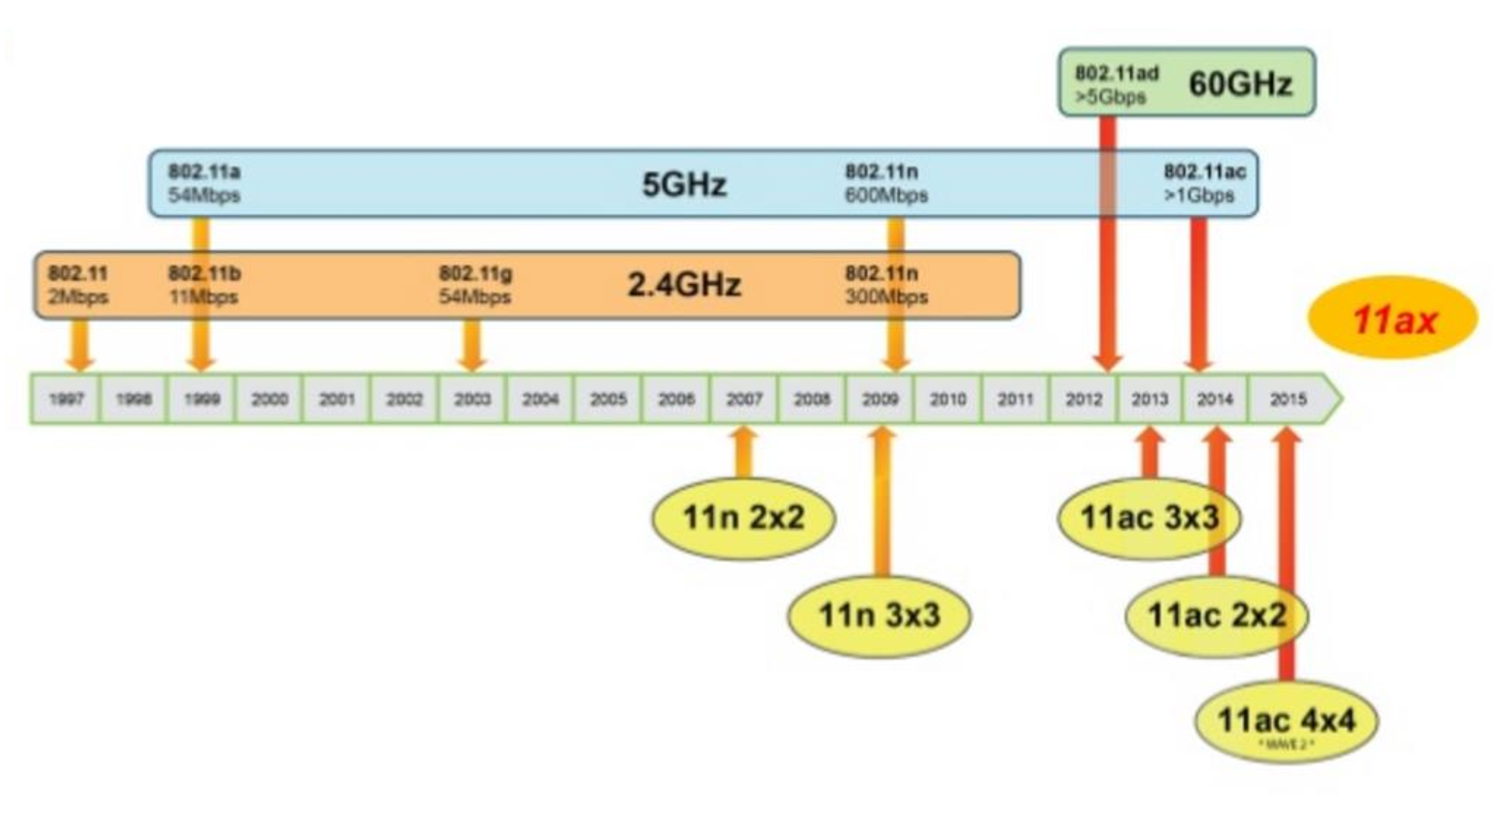
\includegraphics[width=1.0\columnwidth]{figures2/Wi-Fi-evolution.pdf}
	\caption{IEEE 802.11/Wi-Fi Standard Evolution.}
	\label{figs:Wi-Fi-evolution}
\end{figure}

The original 802.11 standard (introduced in 1997) can support only $1$ or $2$ Mbps which is quite low. It was aimed to provide an alternative to and/or to replace wired Ethernet connectivity. The WLAN rate is then significantly improved with IEEE 802.11b and IEEE 802.11a rectified in 1999. The 802.11b, considered as the \textit{first generation} WLAN technology, features two well-known spread spectrum technologies to distribute packets over a wireless medium: Frequency-Hopping Spread Spectrum (FHSS) and Direct-Sequence Spread Spectrum (DSSS) that are still in use by most wireless networks today. It operates in $2.4$ GHz frequency band and can support a maximum data rate of $11$ Mbps. The IEEE 802.11a - the \textit{second generation} WLAN technology - employs the Orthogonal Frequency Division Multiplexing (OFDM) technology to enable a higher data rate of $54$ Mbps. Using the $5$ GHz band, this standard has a significant advantage when the $2.4$ GHz band is heavily crowded. Next, the \textit{third generation }WLAN technology - the IEEE 802.11g - was released in 2003. It operates in the $2.4$ GHz band (as the IEEE 802.11b) and uses OFDM to match the $54$ Mbps data rate achieved by the 802.11a. The 802.11e was then introduced in 2005 to enhance the 802.11a and b with the support of QoSs. It operates at radio frequencies of up to $5.8$ GHz and is most suitable for networks with multimedia applications. In order to further boost the data rate, in 2007, the 802.11n using Multiple Input Multiple Output (MIMO) technology was introduced. It is considered as the \textit{fourth generation} WLANs, using both $2.4$ and $5$ GHz frequency bands and can support up to $600$ Mbps. The 802.11n is now becoming the dominant deployed standard.

The demand for higher throughput over the wireless medium escalated in the late 2000s, driven by mass adoption of smart phones, tablets, and video on demand services such as YouTube and Netflix. To address this, the 802.11ac, also known as the \textit{fifth generation} or gigabit Wi-Fi, was approved in 2014. It operates only in $5$ GHz band, incorporating the enhanced air interface of 802.11n with wider bandwidth, more MIMO streams, and high-density modulation to support at least $1$ Gbps. This standard is now incorporated in many mainstream Wi-Fi products. The 802.11ad is another gigabit Wi-Fi which was introduced in 2012, operating in the unlicensed $60$ GHz band and offering much higher transfer rates than previous 802.11 standards (its theoretical maximum transfer rate is up to $7$ Gbps). Technology based on the 802.11ad standard can supplement existing wireless networks for high-definition video streaming, offering the ability to offload heavy demands on $2.4$ and $5$ GHz that other 802.11 standards are operating on. The 802.11ax - the successor to the 802.11ac and also called  High-Efficiency Wireless (HEW) - is currently at its early stage of development that has the goal of providing $10$ Gbps in both $2.4$ and $5$ GHz bands. This new standard implements several technologies to enhance the efficiency of channel utilization and is therefore expected to provide users with consistent and reliable data throughput in crowded wireless environments. One of the biggest enabling technologies of this efficiency is multi-user technology, both in the form of Multi-User MIMO (MU-MIMO) and Multi-User OFDMA (MU-OFDMA).


\section{IEEE 802.11 CSMA/CA}
\label{csma}

Despite that fact that many generations of IEEE 802.11 has been developed to enhance data rates and support additional features as presented in previous section, they basically share the same MAC mechanism which dictates how multiple devices can share the radio channel. In a nut shell, the 802.11 standard defines two operating modes. In the infrastructure mode, wireless clients are directly connected to an Access Point (AP) in the star topology. APs are connected to a distribution network, usually wired LANs, for Internet connection. In the ad-hoc mode, clients are connected to one another without any AP. While ad-hoc mode is only used in a limited number of scenarios, the infrastructure mode is deployed in almost all Wi-Fi networks. The MAC layer for the infrastructure Wi-Fi networks is composed of two radio channel coordination functions: distributed coordination function (DCF) and point coordination function (PCF).

\subsection{PCF and DCF}
\label{pcf-dcf}

DCF is a contention-based LBT mechanism called \textit{Carrier Sense Multiple Access with Collision Avoidance (CSMA/CA)} that \textit{works in an entirely distributed manner without any coordination}. With CSMA/CA, stations (STAs) independently perform carrier sensing and back-off procedures to compete for the channel access. DCF is a mandatory MAC function and implemented in all IEEE 802.11/Wi-Fi devices. CSMA/CA is focused in this chapter and its technical details will be presented in section \ref{collision-avoidance}.

PCF is built on the top of DCF. It aims to support applications that require near real-time services. Basically, PCF splits the time into periodic interval called beacon intervals, each of which is composed of contention-free period (CFP) and contention period (CP). \textit{CFP requires coordination from the access point (AP)} and allocates resources to STAs using polling mechanism. Specifically, AP maintains a list of registered PCF-enabled STAs and polls each of them using CF-Poll frames. Only after a STA is polled, it can start its data transmission. In case the polled STA does not have any frames to send, then it must transmit null frame. Channel access in CP of PCF is handled by CSMA/CA protocol. PCF is specified as an optional MAC function and has not been widely implemented due to its complexity.

The timing of PCF and DCF of IEEE 802.11 is sketched in Fig. \ref{figs:802-11-PCF-DCF}. Within a given beacon interval, the start and end of CFP are marked by beacon and CF-End control frames, respectively. CP follows CFP and is terminated by a beacon frame of the next beacon interval. 


\begin{figure}[!t]
	\centering
	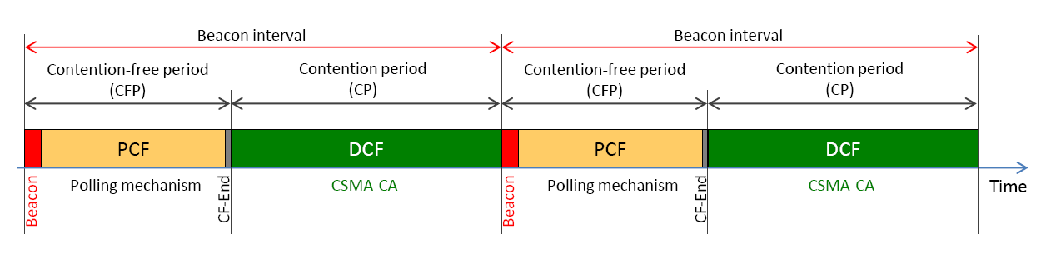
\includegraphics[width=1.0\columnwidth]{figures2/802-11-PCF-DCF}
	\caption{PCF and DCF in IEEE 802.11.}
	\label{figs:802-11-PCF-DCF}
\end{figure}

\subsection{Basic Medium Access}
\label{basic-medium-access}

The LBT mechanism employed by the IEEE 802.11/Wi-Fi CSMA/CA basically follows the same philosophy of carrier sensing protocol family. When a STA needs to transmit a new frame, the channel is sensed and if it is found idle the frame is transmitted immediately. This simple mechanism is very effective when the medium is not heavily loaded since it allows STAs to transmit with a minimum delay. However, it cannot prevent channel access collisions when multiple STAs detect free channel and decide to transmit their frames at the same time. As a result, in addition to this basic channel access, a number of important mechanisms are mandated in CSMA/CA.

\begin{figure}[!t]
	\centering
	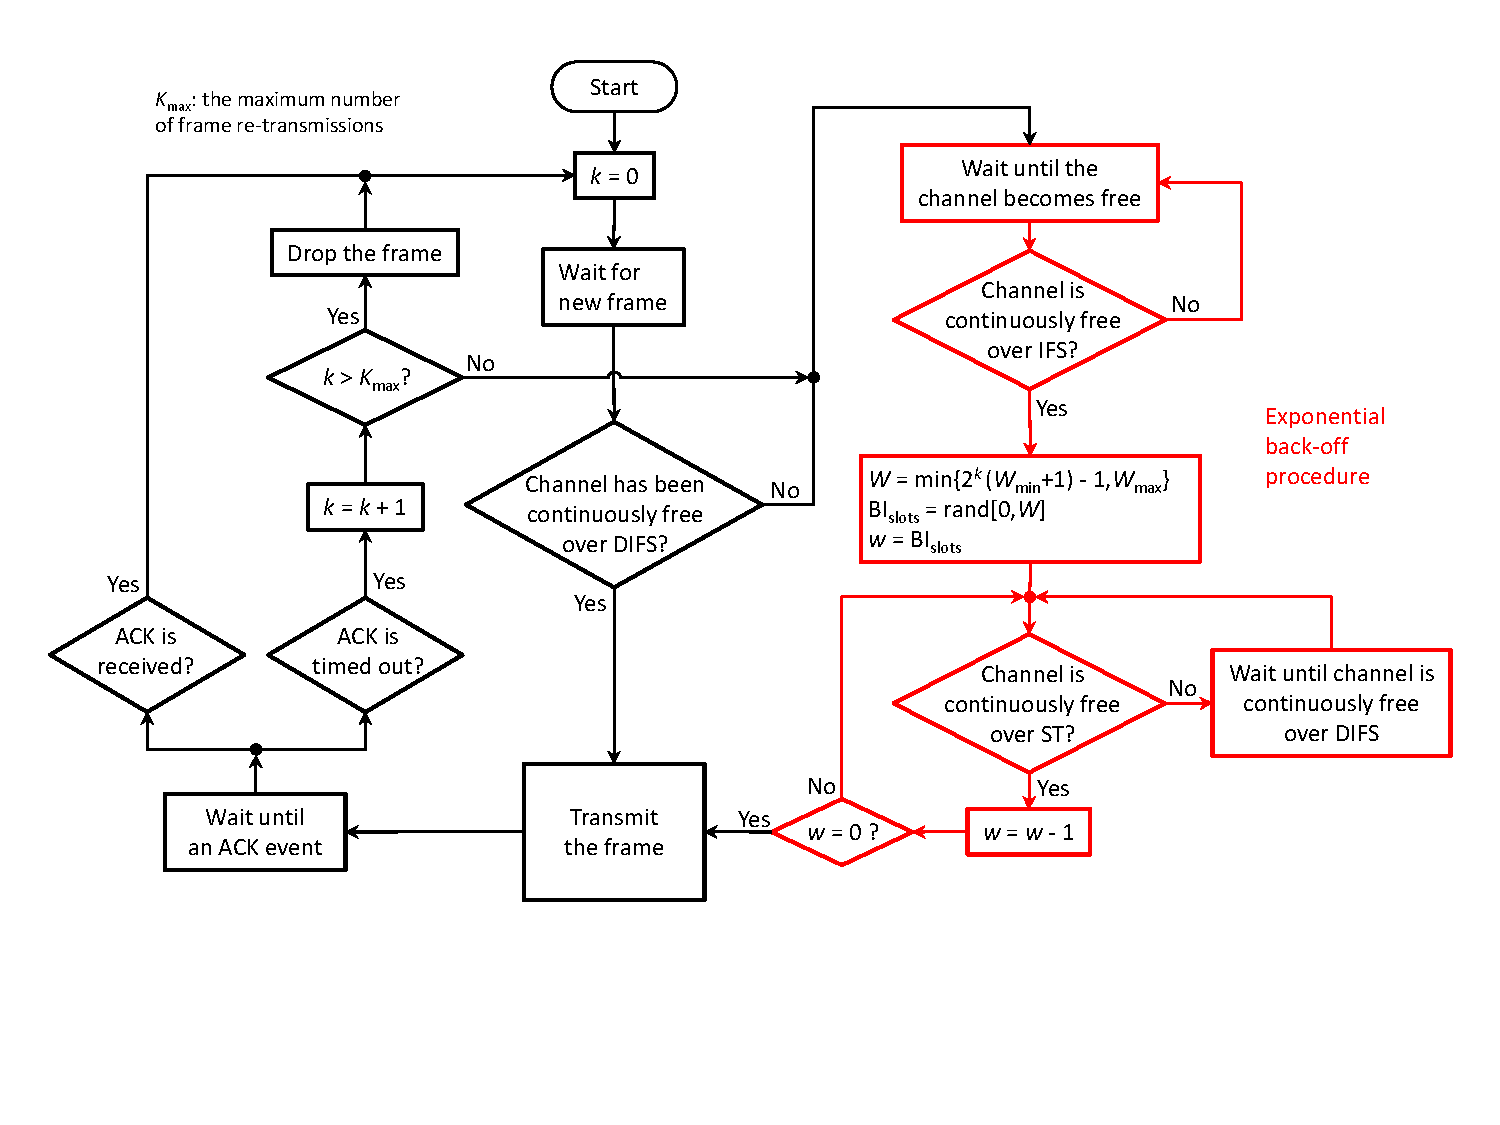
\includegraphics[width=1.0\columnwidth]{figures2/CSMA-CA-flowchart}
	\caption{Simplified flowchart of CSMA/CA.}
	\label{figs:CSMA-CA-flowchart}
\end{figure}


\subsection{Medium Access with Collision Avoidance}
\label{collision-avoidance}

Since it is difficult to detect collisions at a wireless receiver, the IEEE 802.11 protocol tries to avoid collisions rather than detect and recover from collisions. This means that CA mechanisms are mandated to reduce the collision probability at the points where collisions would most likely occur. Specifically, most collisions happen when the medium has become idle (as indicated by CS function) after a busy state: several STAs could have been waiting for the medium to be available again, then all transmit at the same moment the medium is detected free. This situation necessitates a ``random'' back-off procedure to resolve medium contention conflicts. Also, the use of various Inter-Frame Spaces (IFSs) helps to resolve the problem. The CSMA/CA protocol is outlined as follows.

\begin{figure}[!t]
	\centering
	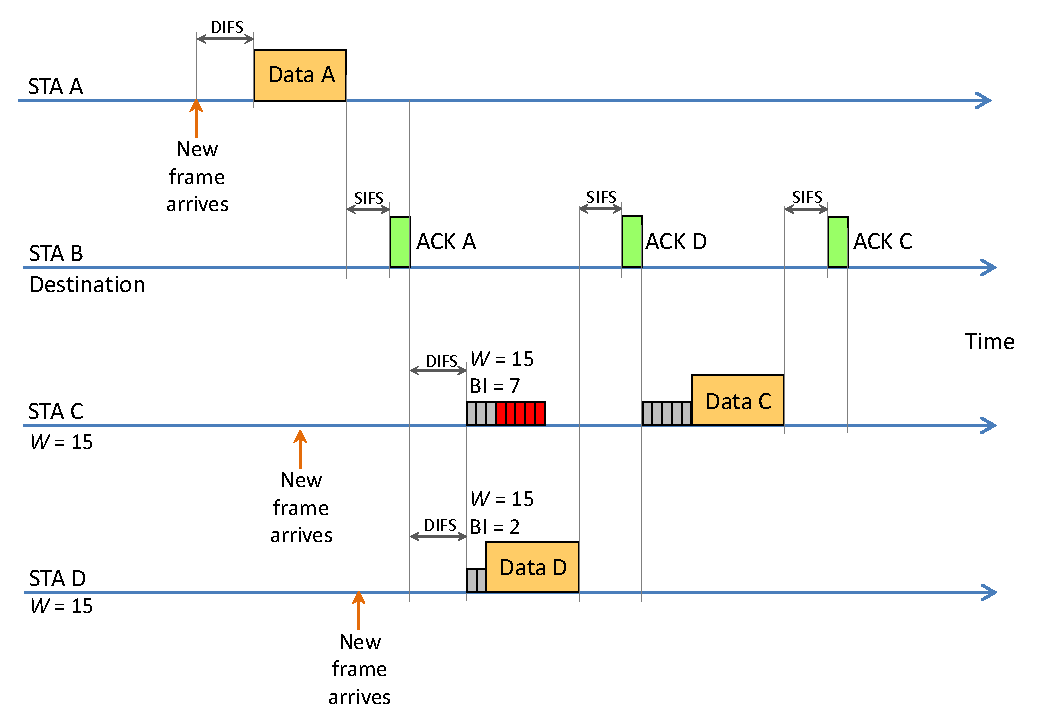
\includegraphics[width=0.9\columnwidth]{figures2/CSMA-CA-back-off-no-collision}
	\caption{CSMA/CA: An example of back-off procedure when there is no collision.}
	\label{figs:CSMA-CA-back-off-no-collision}
\end{figure}

When a STA needs to transmit a new frame, if the channel has been continuously free over a Distributed IFS (DIFS) interval, it transmits immediately. Otherwise, STA defers its transmission until the channel becomes available. Then if the channel is detected to be continuously free over a Distributed IFS (DIFS) interval, the STA will initiate the back-off procedure to further defer its transmission over a random time interval. The back-off procedure starts with the selection of a random ``slotted'' back-off interval $\mathrm{BI_{slots}} = \mathrm{rand}[0,W]$, where $\mathrm{rand}[0,W]$ is a random number uniformly distributed in the range from $0$ to $W$, $W$ is back-off window (when the system is started $W$ is assigned to its minimum value $W_{\min}$). Next, back-off counter $w$ is initialized with $\mathrm{BI_{slots}}$ and decreased every time the medium is idle over a Slot Time (ST). This counter is frozen when a transmission is detected on the medium, and resumed when the channel is detected idle again for a DIFS interval. As soon as $w$ finally reaches zero, the STA transmits its frame. It is important to note that this back-off procedure randomizes the channel access among STAs and thus helps to reduce the chance of collision. It also gives all STAs their fair shares of the channel.

The destination STA, upon receiving a frame correctly, waits for a Short IFS (SIFS) interval immediately after the reception has completed and transmits an ACK frame back to the source STA in order to confirm the correct reception. SIFS is the smallest IFS to give the highest priority channel access to ACK frames. If the source STA receives a confirmation, transmissions of the second and subsequent frames of a fragment burst will use SIFS instead of DIFS. Otherwise, the source STA activates the re-transmission procedure for the lost frame.

When a transmission is lost (due to channel collision when two or more STAs decrease their back-off counter to zero at the same time and transmit their frames at the same time or transmission errors), the contention window $W$ is doubled and applied for the re-transmissions until it reaches a maximum value $W_{\max}$. For the re-transmissions, the back-off procedure is activated after the channel remains idle for an Extended IFS (EIFS) interval. When a frame transmission is successful, contention window $W$ is reset to its minimum value $W_{\min}$. When a maximum number of frame re-transmissions is exhausted, the frame is discarded and $W$ is also reset to its minimum value $W_{\min}$.

\begin{figure}[!t]
	\centering
	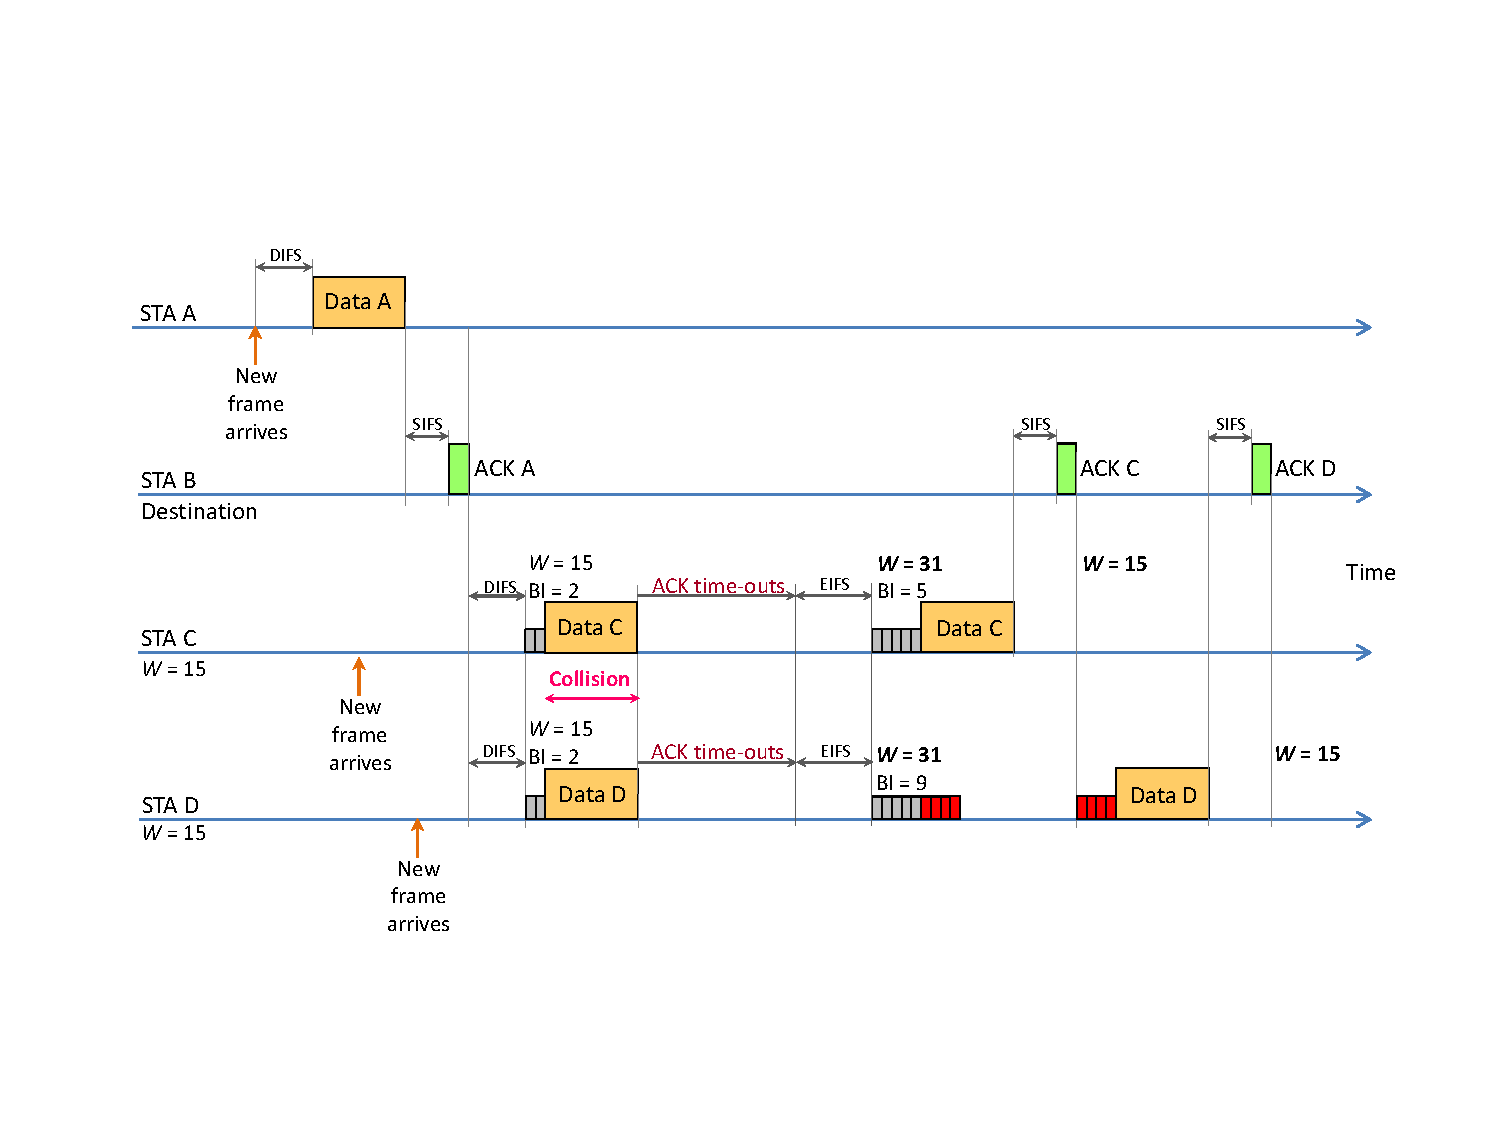
\includegraphics[width=1.0\columnwidth]{figures2/CSMA-CA-back-off-with-collision}
	\caption{CSMA/CA: An example of back-off procedure when there is a collision (the contention window is exponentially increased).}
	\label{figs:CSMA-CA-back-off-with-collision}
\end{figure}

The reason behind the exponential growth of contention window $W$ is explained as follows. When a STA experiences a collision, it has no information on how many STAs are involved in the collision. If there are only few colliding frames, it would make sense to choose the random back-off interval from a small set of small values, i.e., $W$ is small. But if many STAs are involved in a collision, then it makes sense to choose the back-off interval from a larger, more dispersed set of values, i.e., $W$ is large. Otherwise, if several STAs select the back-off interval from a small set of values, more than one STA would choose the same back-off value with high probability. This will result in high probability of collision.

Fig. \ref{figs:CSMA-CA-flowchart} shows the flowchart of CSMA/CA protocol. Figs. \ref{figs:CSMA-CA-back-off-no-collision} and \ref{figs:CSMA-CA-back-off-with-collision} demonstrates the operations of the back-off procedure in two typical scenarios. As visualized in Fig. \ref{figs:CSMA-CA-back-off-no-collision}, by randomly selecting back-off intervals, STAs C and D randomize their channel access to minimize the chance that they transmit their frames at the same time. In case a collision takes place, as shown in Fig. \ref{figs:CSMA-CA-back-off-with-collision}, STAs C and D double their contention windows to further increase the randomness in their back-off interval generations.

Here are some illustrative values of CSMA/CA operation parameters: ST = $20$ $\mu$s, SIFS = $10$ $\mu$s, DIFS = SIFS + $2\times$ST = $50$ $\mu$s, EIFS = Transmission time of ACK frame at lowest physical mandatory rate + SIFS + DIFS, $W_{\min}$ = $31$, and $W_{\max}$ = $1023$. Contention window of the initial transmission attempt is $W(0)=W_{\min}=31$. Contention window of the $k$-th re-transmission is $W(k)=\min\{2^{k}(W_{\min}+1)-1, W_{\max}\}$, where $k \in \{1,2, ..., K_{\max}\}$, $K_{\max}$ is the maximum number of re-transmission attempts. Assuming $K_{\max}=7$, then the progression of contention window with frame transmission/re-transmissions is as follows: $W(0)=31$ (the initial transmission attempt), $W(1)=63$ (the first re-transmission attempt), $W(2)=127$ (the second re-transmission attempt), $W(3)=255$ (the third re-transmission attempt), $W(4)=511$, $W(5)=1023$, $W(6)=1023$, and finally $W(7)=1023$. Different IEEE 802.11 physical layer standards could specify different values for these parameters to optimize their operations.

\begin{figure}[!t]
	\centering
	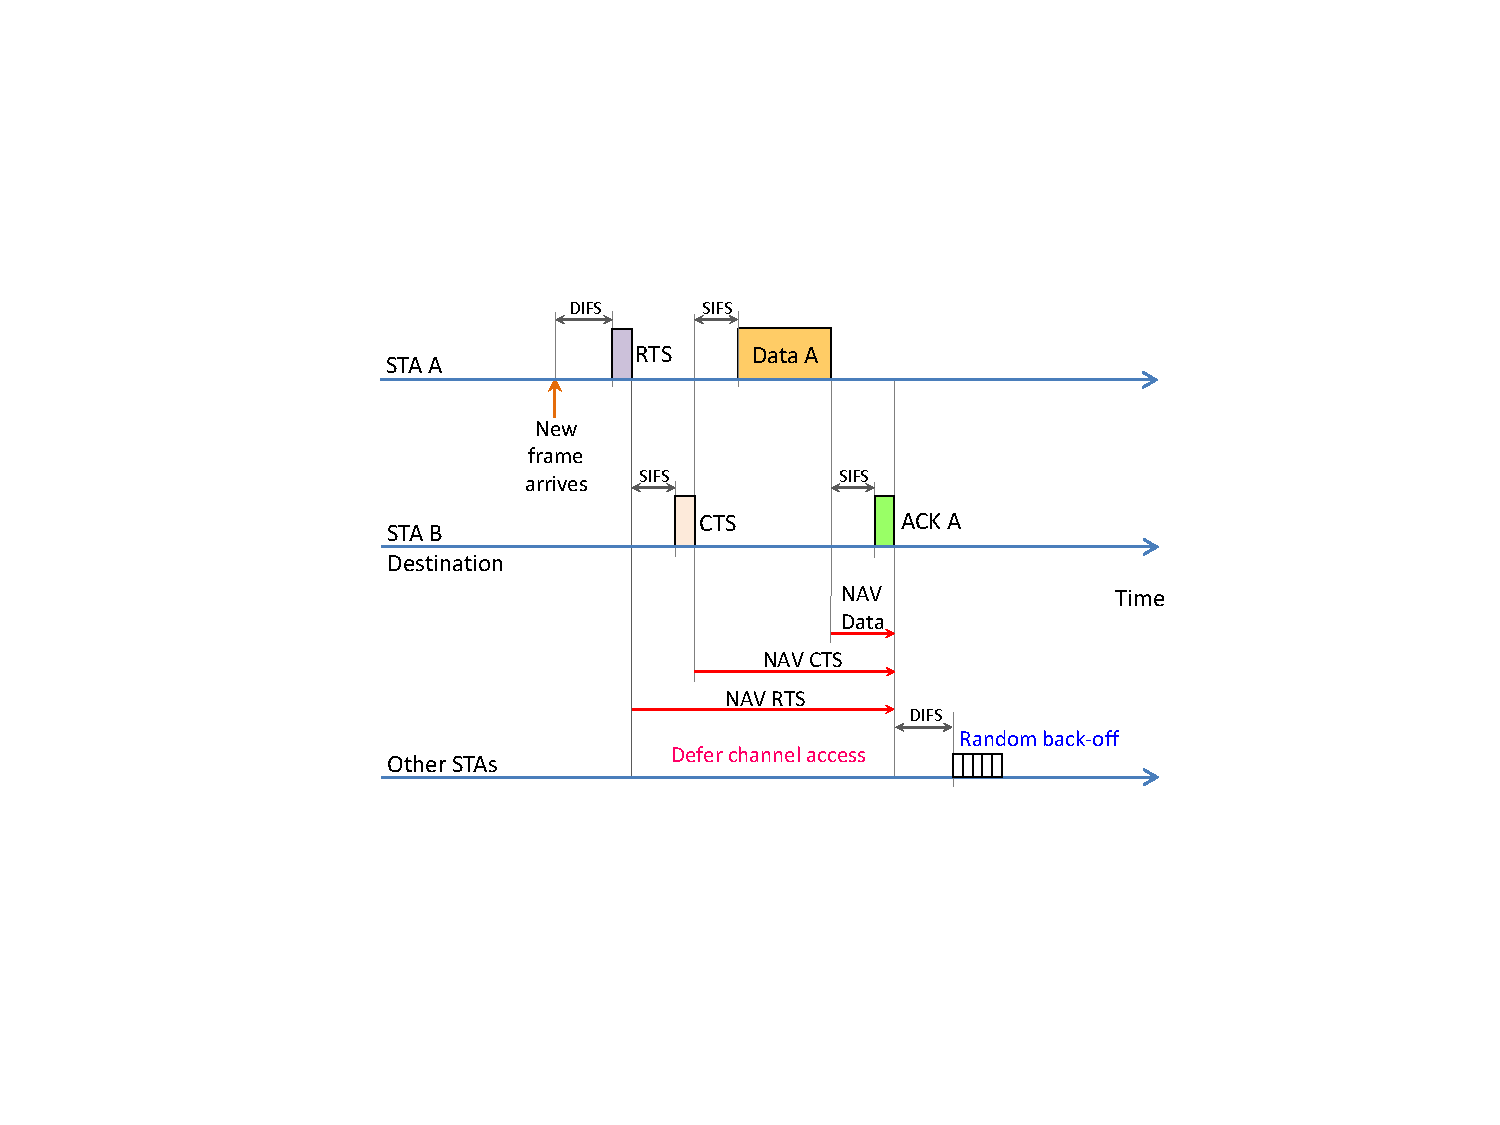
\includegraphics[width=0.65\columnwidth]{figures2/802-11-RTS-CTS-NAV}
	\caption{CSMA/CA enhanced with RTS/CTS handshake and NAV.}
	\label{figs:802-11-RTS-CTS-NAV}
\end{figure}

In order to provide guaranteed reservation of the channel and hence uninterrupted data transmission, CSMA/CA protocol can be enhanced with Request-To-Send (RTS)/Clear-To-Send (CTS) handshake and virtual carrier sense using Network Allocation Vector (NAV). The former is an optional mechanism and only employed for transmissions of long frames (determined by RTS threshold which is typically around $500$ bytes). The latter is a prominent mechanism which is widely used with CSMA/CA protocol.

In RTS/CTS access mode, prior to the data transmission, the source STA will send a RTS frame to announce the upcoming transmission. When the destination STA receives RTS, it will send a CTS frame after a SIFS interval if it is available to receive the data. The source STA is allowed to transmit its data frame only if it receives the CTS frame correctly. The purpose of this RTS/CTS exchange is to clear hidden areas and avoid long collisions. RTS/CTS is illustrated in Fig. \ref{figs:802-11-RTS-CTS-NAV}.

To implement virtual carrier sensing, each STA sends duration information in frame headers. This duration information indicates the amount of time (in microseconds) the medium is to be reserved after the end of the current frame. STAs listening on the wireless medium read the duration fields and set their NAVs, which is an indicator for a STA on how long it must defer from accessing the medium. They count down their NAVs and do not access the channel (even if their physical carrier sense indicates that the channel is free) until NAVs reach zero. NAV is illustrated in Fig. \ref{figs:802-11-RTS-CTS-NAV}. As can be seen, the NAV field in RTS frame allows CTS, data, and ACK frames to be completed (or allows only CTS frame to be completed in some implementations). The NAV in CTS frame allows data and ACK frames to be completed. Finally, the NAV in data frame allows the ACK frame to be completed.


\section{IEEE 802.11e EDCA}
\label{80211e}

The biggest limitation of IEEE 802.11 CSMA/CA is its lack of capability to differentiate frames in terms of channel access priorities for different applications. As a result, the IEEE developed enhancements in IEEE 802.11e to both coordination modes to facilitate QoS. The following sections will present details of 802.11 CSMA/CA protocol and its enhancements introduced in 802.11e. 

The enhancement to DCF, namely Enhanced Distribution Coordination Function (EDCF), introduces the concept of access categories (ACs). Each STA has four kinds of ACs that define four respective priority levels to differentiate the channel access probability for different traffic types. With EDCF, high priority traffic has a higher chance of being sent than low priority traffic: a STA with high priority traffic waits a little less before it sends its packet, on average, than a STA with low priority traffic. This is accomplished by using a shorter contention window and shorter Arbitration Interframe Space (AIFS).

IEEE 802.11e extends the polling mechanism of PCF with the Hybrid Coordination Function (HCF). The HCF controlled channel access (HCCA) works similarly to PCF. However, in contrast to PCF, in which the interval between two beacon frames is strictly divided into two periods of CFP and CP, the HCCA allows CFPs to be initiated at almost any time during a CP. This kind of CFP is called a Controlled Access Phase (CAP) in 802.11e. A CAP is initiated by the AP whenever it wants to send a frame to a STA or receive a frame from a STA in a contention-free manner. In fact, the CFP is a CAP too. During a CAP, the Hybrid Coordinator (HC), which is also the AP, controls the access to the medium using polling mechanism. During the CP, all STAs function in EDCA. The second difference with PCF is that Traffic Class (TC) and Traffic Streams (TSs) are defined. This means that HC is not limited to per-station queuing and can provide a kind of per-session service. Also, HC can coordinate these streams or sessions in any fashion it chooses (not just round robin). Moreover, STAs give information about the lengths of their queues for each TC. HC can use this information to give priority to one STA over another, or better adjust its scheduling mechanism.

IEEE 802.11e additionally introduces the concept of transmission opportunity (TXOP). A STA which obtains medium access must not utilize radio resource for duration longer than a limit specified by TXOP. The use of TXOPs reduces the problem of low-rate STAs gaining an inordinate amount of channel time in the conventional 802.11 DCF MAC. Another enhancement is that a STA is only allowed to initiate a frame exchange if it can complete the exchange before the start of the next beacon interval.
\subsection{QoS Provisioning Mechanisms}
\label{qos}

\subsection{EDCA and HCCA}
\label{edca-hcca}

Basic operations of HCCA are illustrated in Fig. \ref{figs:802-11e-HCCA}. HCCA is generally considered as the most advanced and complicated coordination function. With HCCA, QoS can be configured with great precision. QoS-enabled STAs have the ability to request specific transmission parameters (data rate, jitter, etc.), which should allow advanced applications like voice over IP (VoIP) and video streaming to work more effectively on Wi-Fi networks. However, due to its complexity and signaling overhead, HCCA has not been widely implemented.

It can be seen IEEE 802.11 CSMA/CA is the most fundamental protocol for medium access in WLANs. In fact, IEEE 802.11e EDCA is primarily designed based on CSMA/CA. As a result, in-depth knowledge on medium access mechanisms employed by this protocol is imperative to unde
\begin{figure}[!t]
	\centering
	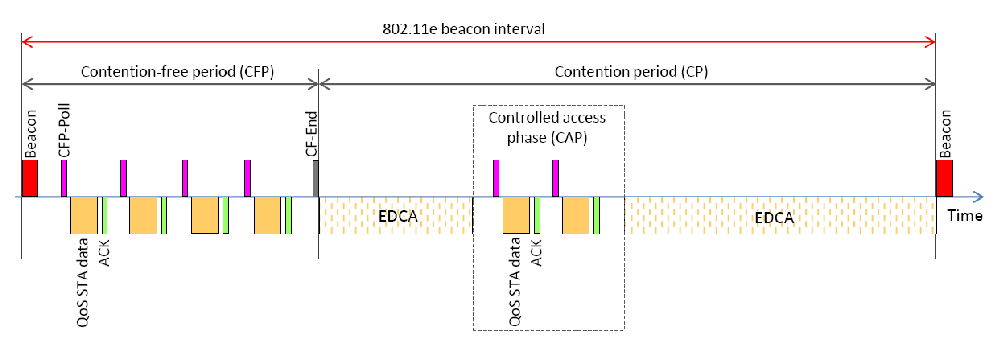
\includegraphics[width=1.0\columnwidth]{figures2/802-11e-HCCA}
	\caption{HCCA in IEEE 802.11e.}
	\label{figs:802-11e-HCCA}
\end{figure}


\section{Important Observations on CSMA/CA}
\label{csmaca-obs}

It is important to note that IEEE 802.11 CSMA/CA is specified with a few key additional features that go beyond LBT requirements specified by ETSI \cite{LBT-ETSI-2014}. \textit{First}, a Wi-Fi device defers to signals that are much weaker than the minimum level required by ETSI. ETSI LBT requires a transmitter to defer if the received energy is above $-60$ dBm (for $20$ MHz), while Wi-Fi defers if the received energy is above $-62$ dBm (this level is referred to as the energy detect threshold, or ED for short) or if a valid Wi-Fi preamble is detected. Wi-Fi's ED threshold is nearly the same as ETSI's LBT threshold, but Wi-Fi preamble detection is required to work to at least $-82$ dBm, and in reality works to $-90$ dBm or lower in most products. Hence, Wi-Fi devices defer to other Wi-Fi transmissions much more conservatively (i.e., at a much larger distance) than a device which only meets ETSI requirements. \textit{Second}, Wi-Fi goes beyond the ETSI requirements in specifying how long a device must wait after the on-air energy falls below the threshold before initiating a transmission. \textit{Third}, when a collision is detected, Wi-Fi employs exponential back-off rule that doubles the contention window size and thus significantly increases the random back-off time in order to avoid future collision.

%%%%%%%%%%%%%%%%%%%%%%%% referenc.tex %%%%%%%%%%%%%%%%%%%%%%%%%%%%%%
% sample references
% %
% Use this file as a template for your own input.
%
%%%%%%%%%%%%%%%%%%%%%%%% Springer-Verlag %%%%%%%%%%%%%%%%%%%%%%%%%%

\begin{thebibliography}{99.}%
\bibitem{wifi-alliance}``Wi-Fi® device shipments to surpass 15 billion by end of 2016'', Online, {Wi-Fi}  Alliance. Available:  \url{{ttp://www.wi-fi.org/news-events/newsroom/wi-fi-device-shipments-to-surpass-15-billion-by-end-of-2016}}.
\bibitem{80211}``{IEEE Standard for information technology--Telecommunications and information exchange between systems Local and metropolitan area networks--Specific requirements Part 11: Wireless LAN medium access control (MAC) and Physical Layer (PHY) specifications},'' \emph{{IEEE Std 802.11-2012 (Revision of IEEE Std 802.11-2007)}}, March 2012.
\bibitem{80211ac}``{IEEE Standard for information technology--Telecommunications and information exchange between systems Local and metropolitan area networks--Specific requirements Part 11: Wireless LAN medium access control (MAC) and Physical Layer (PHY) specifications}--Amendment 4: Enhancements for very high throughput for operation in bands below 6 GHz,'' \emph{{IEEE Std 802.11ac-2013 (Revision of IEEE Std 802.11-2007)}}, December 2013.
\bibitem{80211ad}``{IEEE Standard for information technology--Telecommunications and information exchange between systems Local and metropolitan area networks--Specific requirements Part 11: Wireless LAN medium access control (MAC) and Physical Layer (PHY) specifications amendment 3: Enhancements for very high throughput in the 60 GHz band},'' \emph{{IEEE Std 802.11ad-2012 }},  December 2012.
\bibitem{ieee-history}{J. Berg}, ``The  IEEE  802.11  standardization  – Its  history,  specifications,  implementations,  and  future''; TechnicalReport GMU-TCOM-TR-8,  George  Mason  University. 
Available: \url{\text{http://telecom.gmu.edu/sites/default/files/publications/Berg\_802.11\_GMU-TCOM-TR-8.pdf}}.
\bibitem{LBT-ETSI-2014} \emph{ETSI EN 301 893 V1.7.2 (2014-07): Broadband radio access networks (BRAN);	5 GHz high performance RLAN; Harmonized EN covering the essential requirements of article 3.2 of the R\&TTE Directive}, European Telecommunications Standards Institute Std., 2014.
\end{thebibliography}